\documentclass[a4paper,12pt]{article}
\usepackage[utf8x]{inputenc}
\usepackage[english,russian]{babel}
\usepackage{amsmath}
\usepackage{amsbsy}
\usepackage{graphicx}
\usepackage[normalem]{ulem}
\begin{document}
\begin{flushleft}

\section{Номер 1}

Заметим, что если один из графов состоит лишь из одного ребра и, соответсвенно,
двух вершин, то второй, очевидно, не планарен, так как содержит как подграф 
непланарный $K_{3,3}$.

Тогда заметим, что для каждой компоненты связности из более,
чем двух вершин, покрашенного графа, если он планарен, 
выполняется неравенство $e \leq 3v - 6$. Тогда суммируя и ослабляя неравенства
для компонент: 
$$(e_1 \leq 3v_1 - 6) \land (e_2 \leq 3v_2 - 6) \Rightarrow 
e_1 + e_2 \leq 3(v_1 + v_2) - 12 < 3(v_1 + v_2) - 6$$
Получаем аналогичное неравенство для всего графа. Неравенство справедливо даже если присутствуют
компоненты связности из двух вершин и одного ребра, если только это не одна
единственная компонента связности (1). \sout{(Любопытный проверящий может убедиться
в справедливости данного тривиального утверждения самостоятельно)}.

Действительно: добавляя к графу, удовлетворяющему рассматриваемому неравенству,
граф из одного ребра и двух вершин, мы добавляем одно ребро и две вершины 
(нетривиально), чем не нарушаем неравенство: 
$$ e \leq 3v - 6 \Rightarrow e + 1 \leq 3 (v + 2) - 6$$
Осталось заметить, что несвязный граф уже из двух таких графов 
(одно ребро и две вершины) удовлетворяет рассматриваемому неравенству.
Значит, утверждение (1) верно.

Итак, каждый из наших графов может содержать не более $11$ вершин, а 
рёбер у них в сумме ровно $55$. Но тогда $e_1 + e_2 \leq 3 (v_1 + v_2) - 6 - 6$
$55 \leq 3 \cdot 22 - 12 = 54$. Противоречие. Один из графов не планарен.

\section{Номер 2}

Для полного графа $e = \dfrac{v (v - 1)}{2}$. Тогда очевидно, что начиная
с $v = 5$ неравенство $\dfrac{v (v - 1)}{2} \leq 3v - 6$ не выполняется,
а значит граф не может быть планарным. Планарный граф с $v = 4$ очевиден.
Ответ: $4$.

\section{Номер 3}

\includegraphics[width=4in]{g.png} 

\section{Номер 4}

Принимаем, что звезда в центре имеет правильный пятиугольник. Тогда обозначив
вес его стороны за $b$, а веса остальных отрезков от его вершин до концов звезды
за $a$ из геометрических соображений получим $b = 0.62a$. А из $10a + 5b = 100$
получим $a = 7.63$ и $b = 4.73$.

Применим жадный алгоритм - каждый раз будем выбирать минимальный возможный
путь присоединения новой вершины, учитывая, что нам нужны лишь вершины звезды.

Первый шаг:

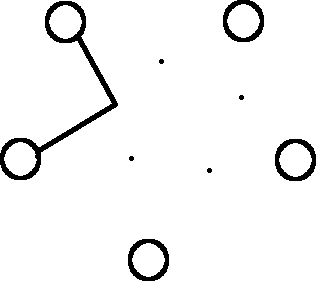
\includegraphics[width=2in]{1.png} 

Второй шаг:

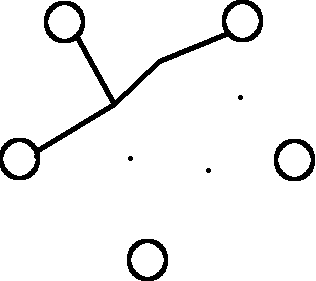
\includegraphics[width=2in]{2.png} 

Третий шаг:

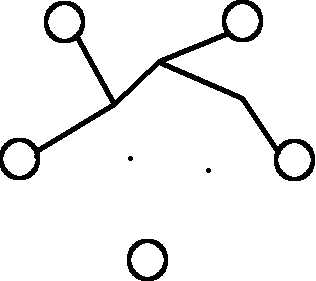
\includegraphics[width=2in]{3.png} 

Четвёртый шаг:

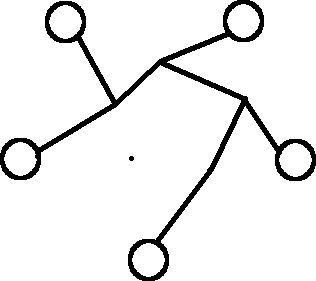
\includegraphics[width=2in]{4.png} 

Вес, который удалось украсть - $5 \cdot a + 2 \cdot b = 47.61$ кг.

\end{flushleft}
\begin{center}
Made with \LaTeX{}, Geany, GIMP and pain
\end{center}
\end{document}
